\section{Exact computation and numerical evidence}\label{sec:computation}

The accompanying program serves two purposes: it checks that independent
finite implementations agree with the definitions, and it illustrates
the asymptotic theorems. All floor and ceiling decisions in the reported
checks use exact integers. Special-function evaluations and plots are
separately identified as numerical diagnostics.

\subsection{Integer and rational exponents}

For integer $m\geq1$, the backward recurrence has the purely integer form
\begin{equation}\label{eq:integer-algorithm}
 q_{k-1}=\left\lfloor
 \frac{k^m q_k+(k-1)^m-1}{(k-1)^m}
 \right\rfloor.
\end{equation}
It computes $T_m(K)$ in $K-1$ arithmetic steps and uses only one current
quotient if no profile is retained. These are counts of arithmetic
operations, not a bit-complexity bound. For fixed $m$, all integer
values involved have $O_m(\log K)$ bits by \cref{eq:global-bound}.

Exact computation is also possible for rational $m=p/q>0$, written in
lowest terms. Given the integer quotient $v=q_k$, the next backward
quotient is the least integer $u$ satisfying
\begin{equation}\label{eq:rational-root}
 u^q(k-1)^p\geq v^q k^p.
\end{equation}
This is an integer-root problem. Let
$N=v^qk^p$, $D=(k-1)^p$, and let $r$ be the integer $q$th root rounded
down of $\lfloor N/D\rfloor$. The desired ceiling is $r$ if
$r^qD=N$, and $r+1$ otherwise. The final comparison is exact, including
the cases where the algebraic expression is an integer.

Independently, the forward quotients satisfy
\begin{equation}\label{eq:forward-quotient}
 Q_1=n,\qquad
 Q_k=\floor{\left(\frac{k-1}{k}\right)^m Q_{k-1}}.
\end{equation}
For $m=p/q$, this is the greatest integer $u$ such that
$u^q k^p\leq Q_{k-1}^q(k-1)^p$. Thus rational exponents can be
checked without ever representing an irrational intermediate $x_k$.

\subsection{Independent checks}

The recorded verification performs the following mathematical checks:
\begin{itemize}
\item For $m=1,2,3$ and every $0\leq n\leq2000$, direct simulation of
the original $x_k$ recurrence agrees with the quotient recurrence and
with the exact backward-threshold interval for the stopping time.
\item For $m=1/2,2/3,3/2,5/3$ and $0\leq n\leq200$, the algebraic
integer-root implementation of the forward process agrees with the
backward survival intervals.
\item All displayed initial terms in the inspected OEIS entries agree:
79 terms for A073047 with offset $1$, and 105 terms each for A082527
and A082528 with offset $0$.
\item For block length $r=3$ and $m=1,2,3$, the exact threshold identity
is checked through $K=200$, and the stopping identity through $n=2000$.
The zero input is checked separately.
\item The finite-product constant enclosures are constructed as exact
fractions for $m=1,2,3,5$ and $j=10,100,1000$, and their stated relative
width is checked exactly.
\end{itemize}
These checks all passed. Their bounds and results are recorded in
\texttt{verification.json}. They audit the finite definitions and
calculations; the infinite statements rest on the preceding proofs.

\subsection{Threshold convergence}

\begin{table}[p]
\centering
\small
\begin{tabular}{rrrl}
\toprule
$m$ & $K$ & Exact $T_m(K)$ & $c_mT_m(K)/K^{m+1}$\\
\midrule
$\tfrac12$ & 10 & 17 & 1.1785908081\\
$\tfrac12$ & 100 & 470 & 1.0304145588\\
$\tfrac12$ & 1000 & 14440 & 1.0011088982\\
$\tfrac12$ & 10000 & 456247 & 1.0002628749\\
$1$ & 10 & 34 & 1.0681415022\\
$1$ & 100 & 3234 & 1.0159910642\\
$1$ & 1000 & 318570 & 1.0008171717\\
$1$ & 10000 & 31833630 & 1.0000829815\\
$2$ & 10 & 244 & 1.2116837876\\
$2$ & 100 & 205688 & 1.0214295693\\
$2$ & 1000 & 201388916 & 1.0000806743\\
$2$ & 10000 & 201457639236 & 1.0004219482\\
$3$ & 10 & 1816 & 1.2284918534\\
$3$ & 100 & 15338896 & 1.0376491616\\
$3$ & 1000 & 148522784144 & 1.0047303434\\
$3$ & 10000 & 1478758856906056 & 1.0003541899\\
$5$ & 10 & 141440 & 1.4628989077\\
$5$ & 100 & 103280328768 & 1.0682174784\\
$5$ & 1000 & 97237370572647616 & 1.0057158031\\
$5$ & 10000 & 96759789128216456247328 & 1.0007762290\\
\bottomrule
\end{tabular}

\caption{Exact backward thresholds and numerical normalizations.
The last column tends to $1$ by \cref{thm:main}; its displayed values
use high-precision evaluation of $c_m$. The full data file also includes
$K=100000$. The exponent $m=1/2$ uses exact integer square roots.}
\label{tab:thresholds}
\end{table}

Table~\ref{tab:thresholds} shows both the correct scale and the irregular
finite errors. For example, for $m=2$ the normalized error at $K=10000$
is larger than at $K=1000$. Neither monotonic convergence nor a
particular rate follows from the theorem or from these samples.

\begin{figure}[tbp]
\centering
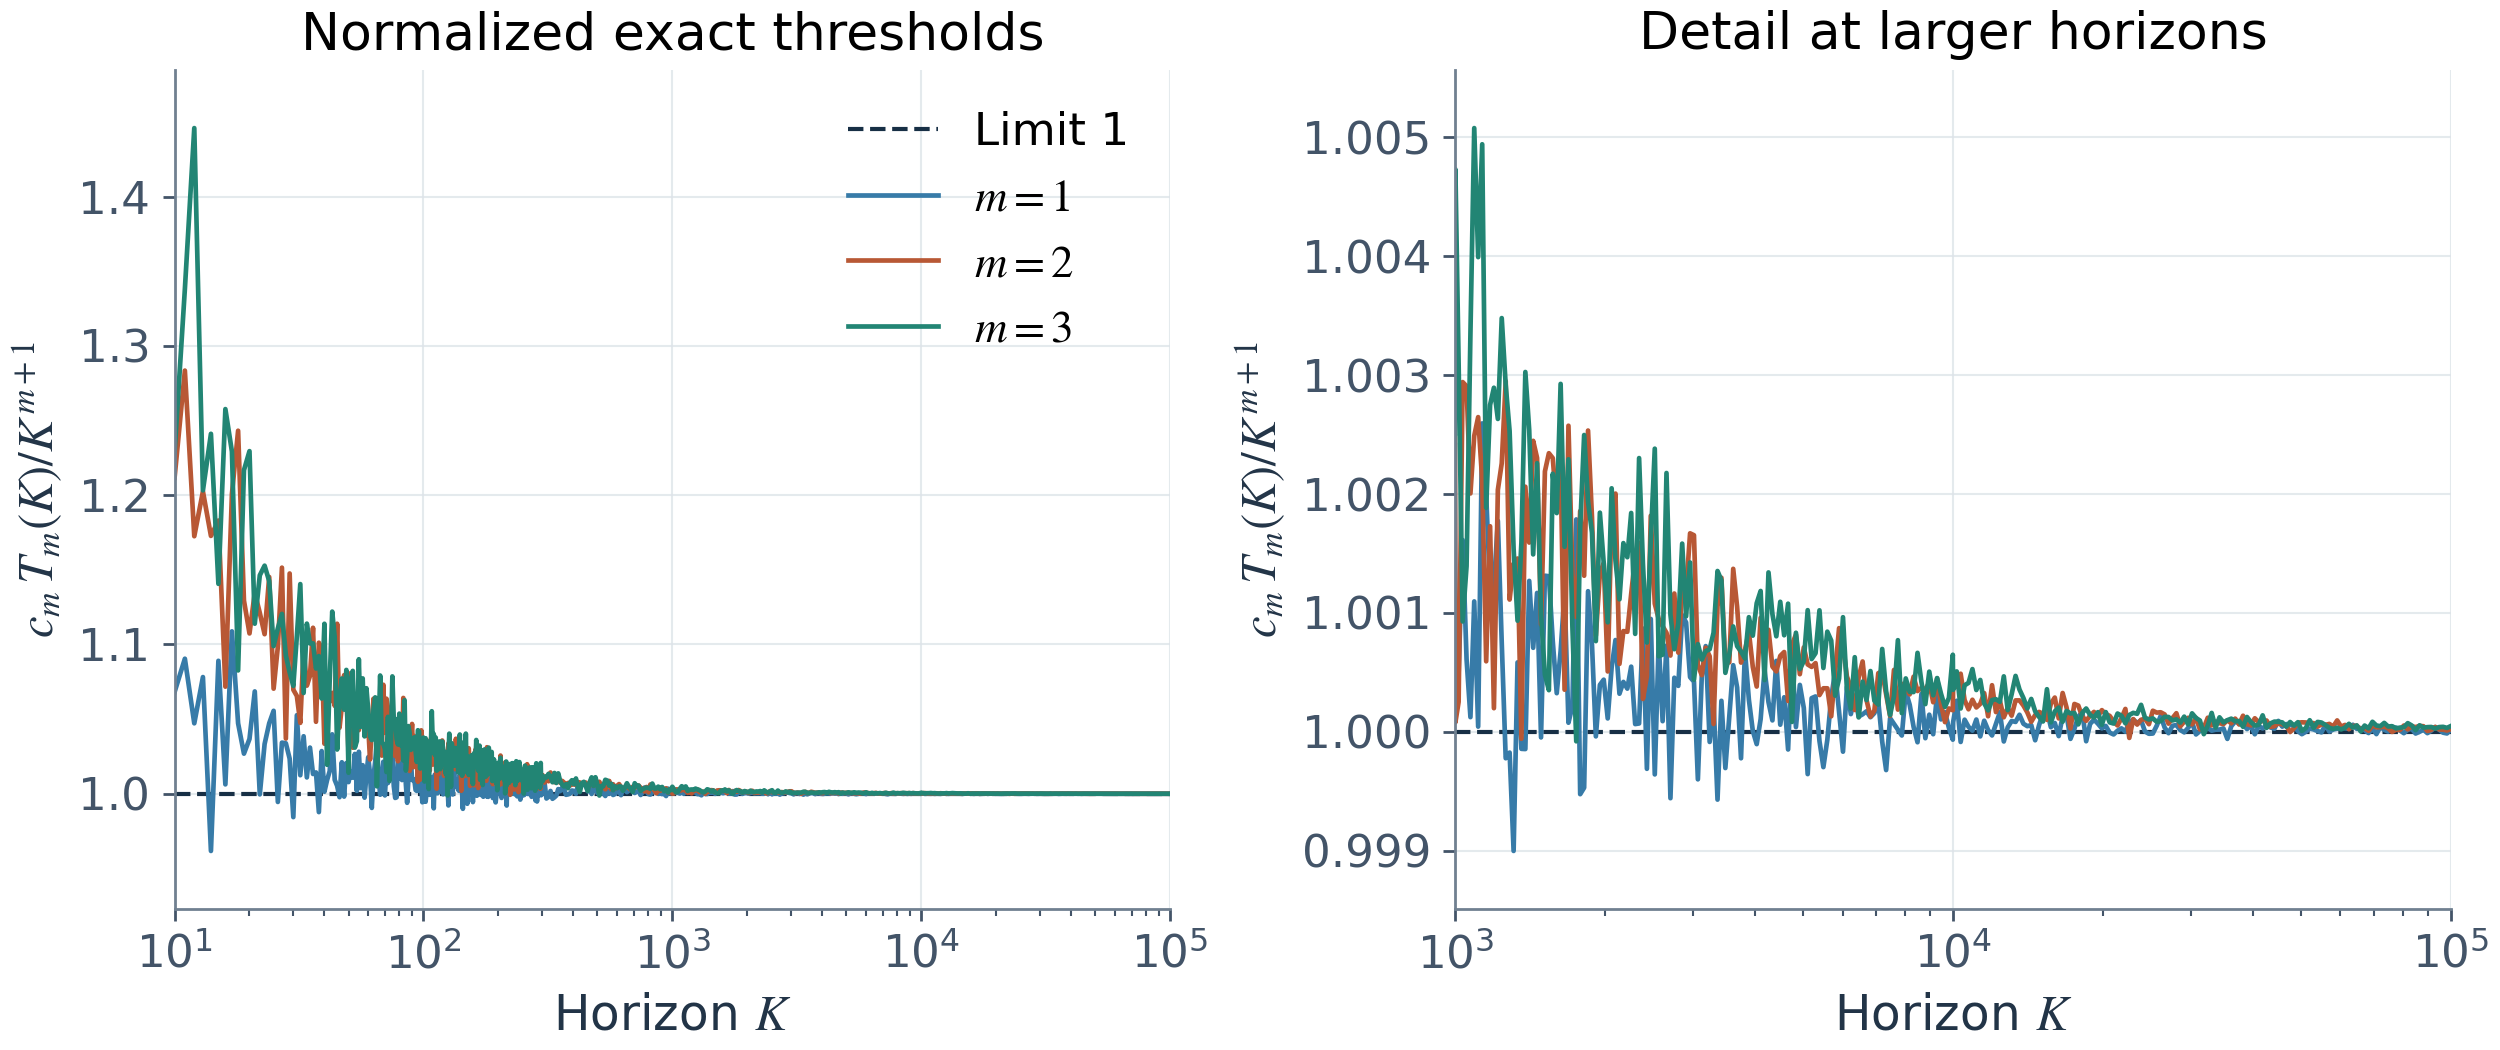
\includegraphics[width=.98\linewidth]{figures/normalized_thresholds.png}
\caption{Normalized thresholds for $m=1,2,3$, calculated by the exact
backward recurrence. The Gamma constants are used only in the
normalization. The irregular excursions illustrate why estimating
a discrete error law requires more than a smooth fitted curve.}
\label{fig:thresholds}
\end{figure}

\subsection{The predicted shapes}

\begin{figure}[tbp]
\centering
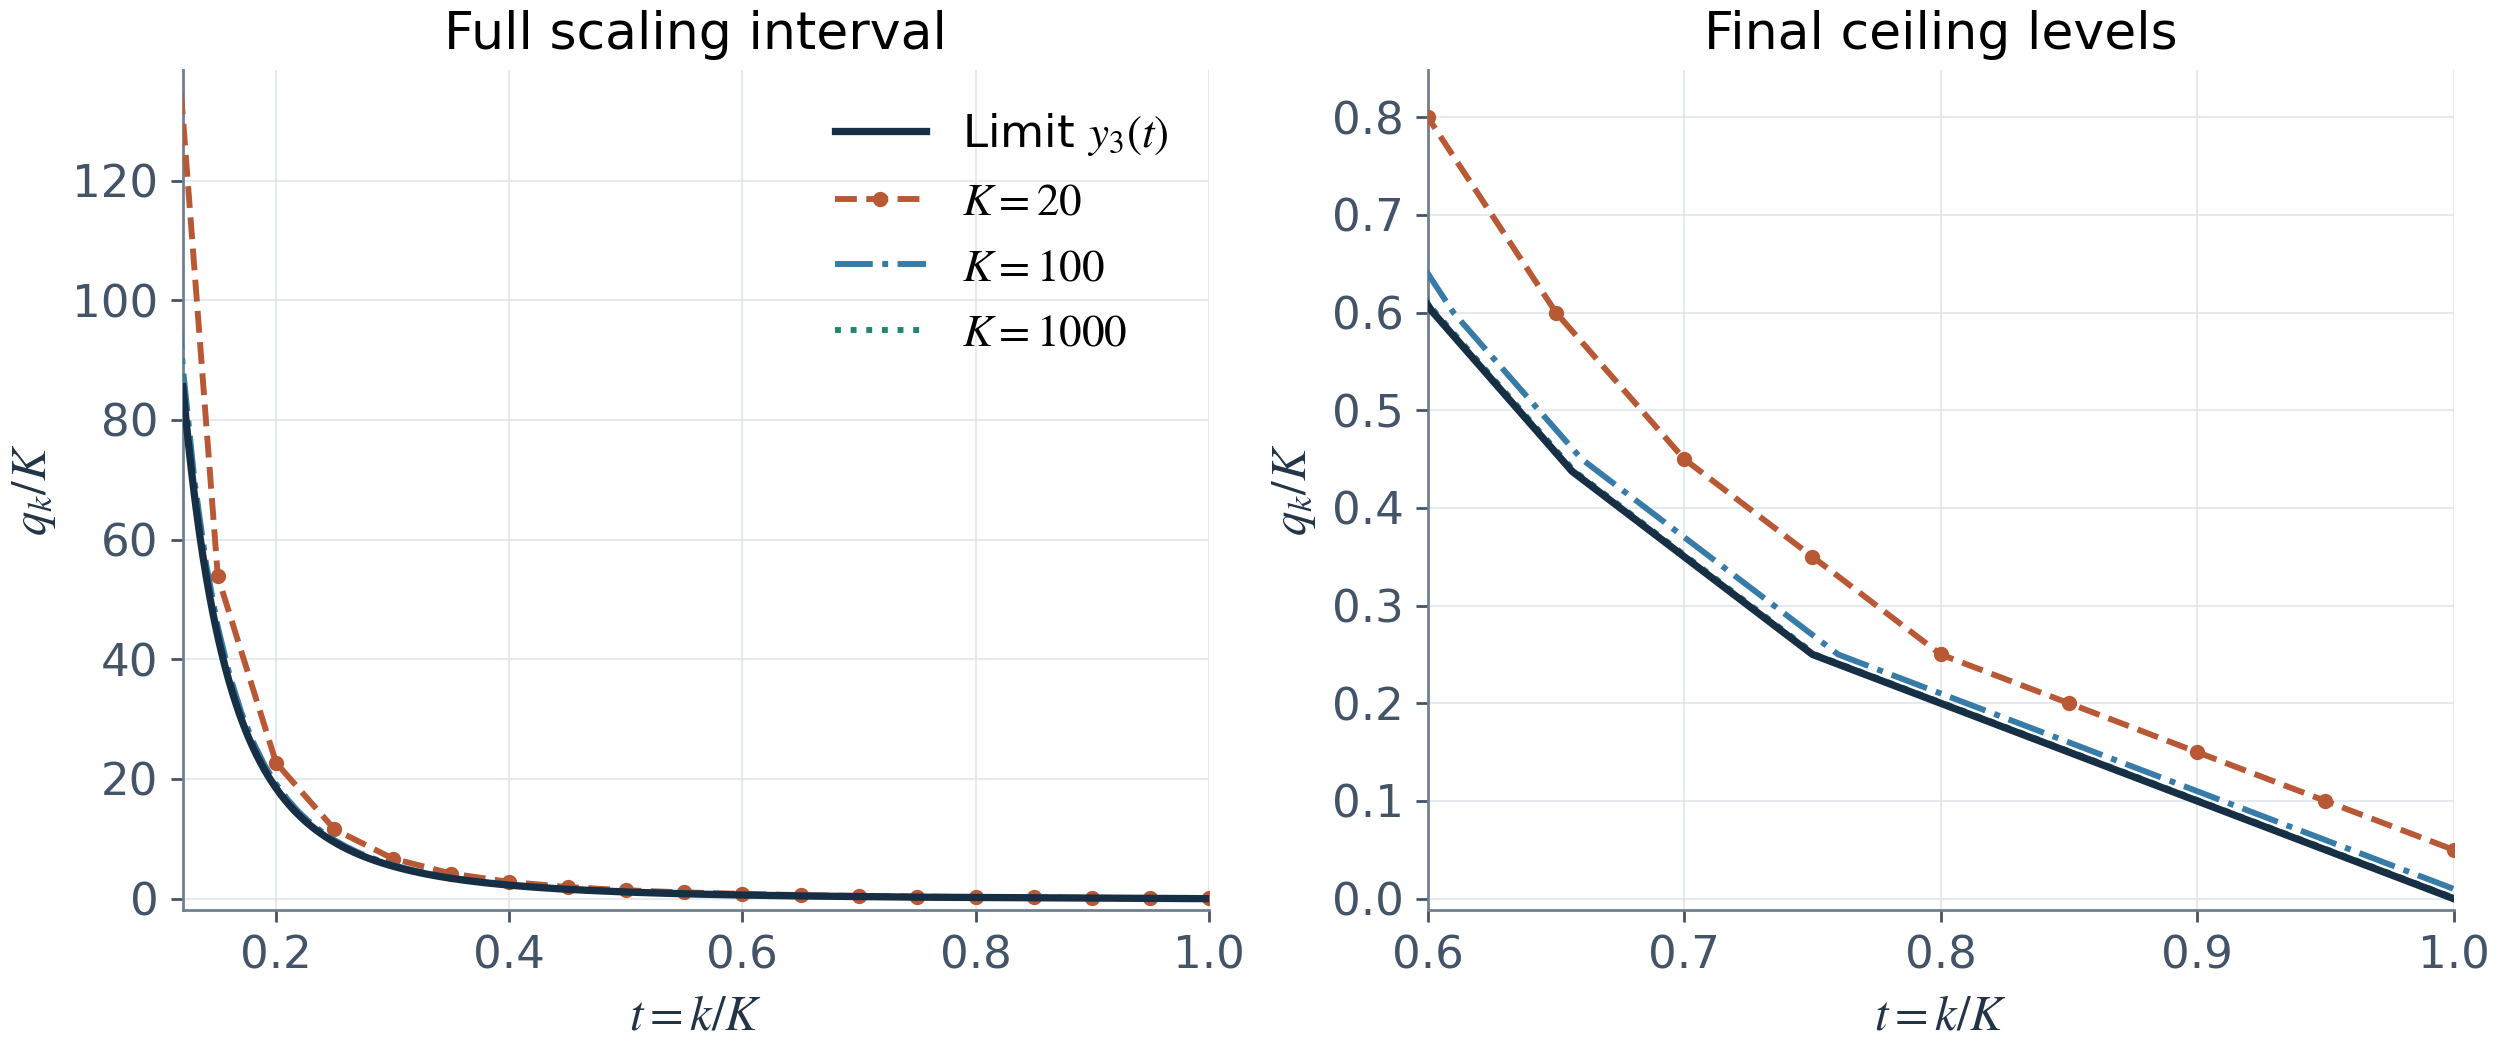
\includegraphics[width=.98\linewidth]{figures/backward_profiles.png}
\caption{The cubic backward quotient profile. Discrete arrays, divided
by their terminal stage $K$, approach the explicit piecewise linear
function $y_3$. The plot stays away from $t=0$, where $y_3$ diverges;
the proof handles that endpoint through weighted tail bounds.}
\label{fig:backward}
\end{figure}

Figure~\ref{fig:backward} directly illustrates the compact convergence
proved in \cref{prop:profile}. Figure~\ref{fig:forward} uses actual
forward trajectories, which were not used to construct the limiting
profile. For the cubic process, the exact stopping indices for initial
values $10^3,10^6,10^9$ are respectively $9,51,287$. The step curves
converge to the continuous weighted profile $F_3$.

\begin{figure}[tbp]
\centering
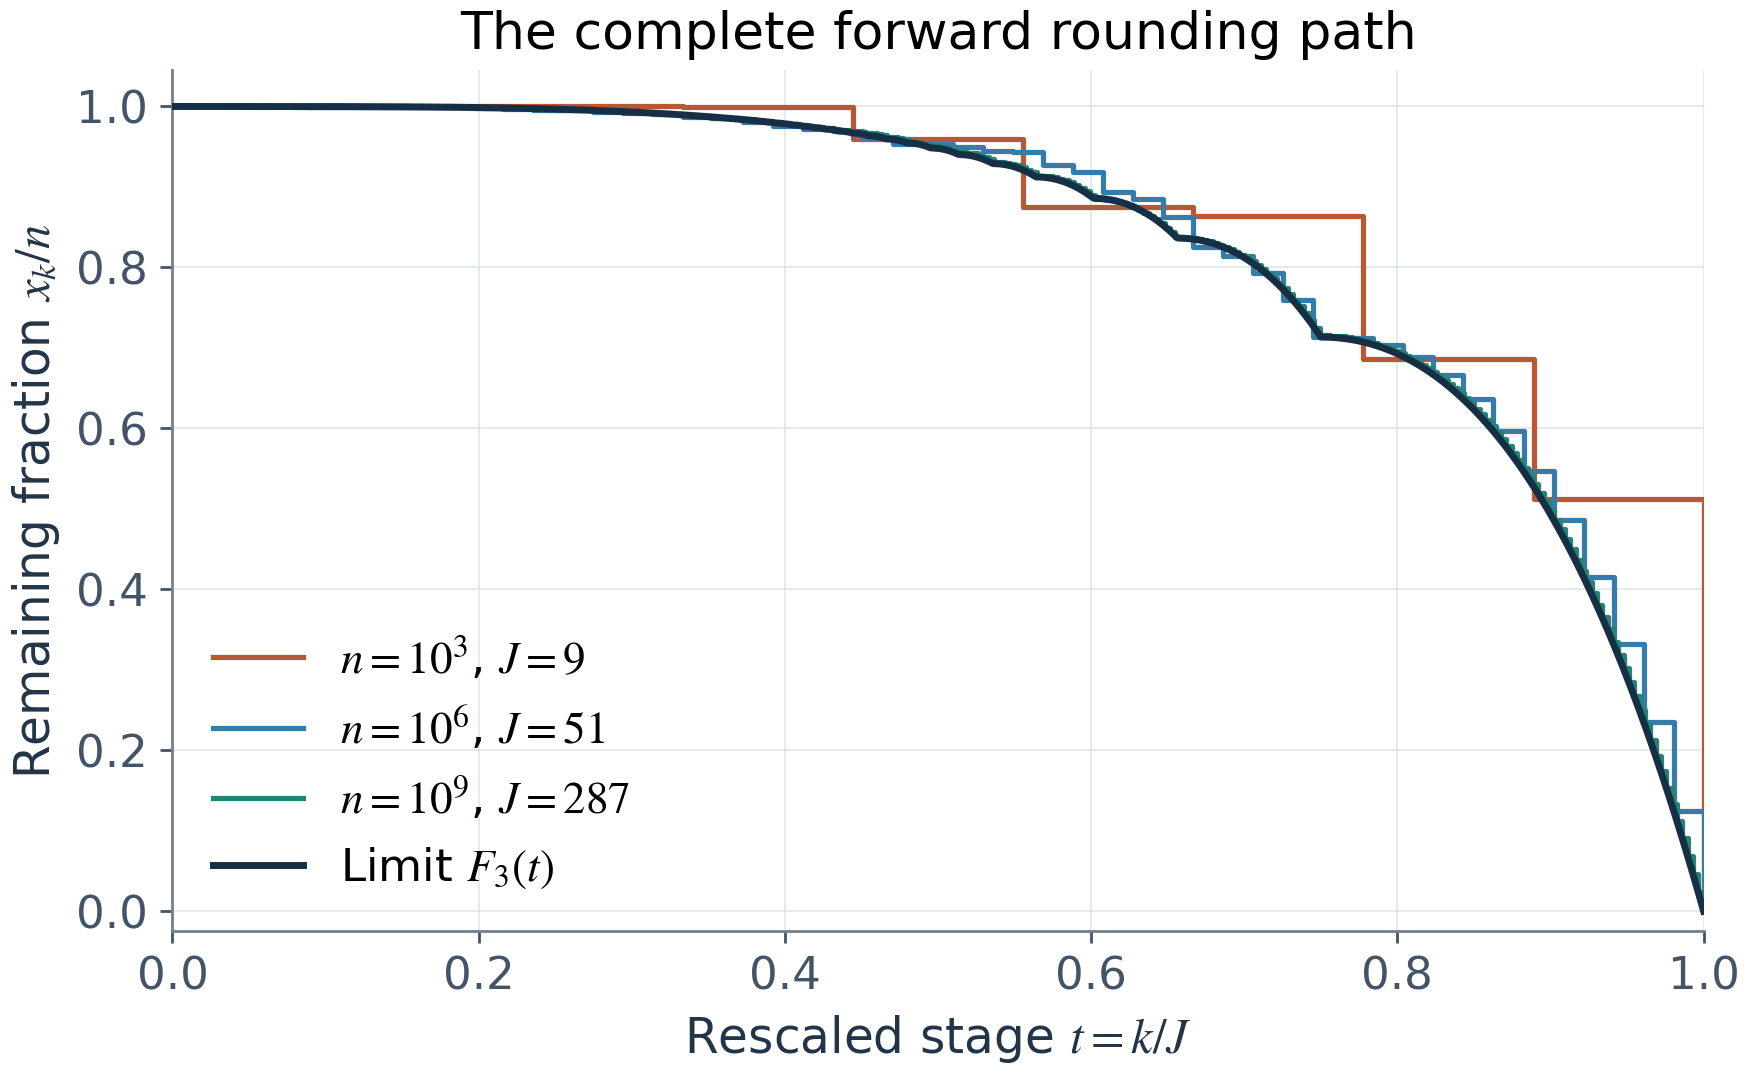
\includegraphics[width=.98\linewidth]{figures/forward_paths.png}
\caption{The fraction of the initial value remaining in three cubic
forward trajectories, with time divided by the exact stopping index.
The limiting curve is $F_3(t)=c_3t^3y_3(t)$. Its continuous value at
$t=0$ is $1$, despite the divergence of the unweighted quotient profile.}
\label{fig:forward}
\end{figure}

\subsection{Certified constant intervals}

\begin{table}[tbp]
\centering
\small
\begin{tabular}{rrrr}
\toprule
$m$ & Lower endpoint & $m\Gamma(m/(m+1))^{m+1}$ & Upper endpoint\\
\midrule
1 & 3.1408077460 & 3.1415926536 & 3.1423781500\\
2 & 4.9642631432 & 4.9659171624 & 4.9675726521\\
3 & 6.7622883375 & 6.7648229810 & 6.7673600538\\
5 & 10.3385883285 & 10.3428938609 & 10.3472038189\\
\bottomrule
\end{tabular}

\caption{Finite-product enclosures from \cref{prop:certificates} at
$j=1000$. The outer decimal endpoints are rounded outward by exact
integer arithmetic, so the displayed intervals retain the enclosure.
The middle column is a numerical evaluation of the exact Gamma formula.}
\label{tab:certificates}
\end{table}

The exact rational numerators and denominators underlying
Table~\ref{tab:certificates} are included in
\begin{quote}\ttfamily
data/constant\_certificates.json
\end{quote}
The table's enclosure is
provided by the theorem and exact endpoint arithmetic. A numerical
comparison of a Gamma evaluation with those intervals is an additional
consistency check, not the basis of their certification.

\subsection{Reproduction and formalization}

The archive includes the LaTeX source, this PDF, the figures, the Python
program, its dependency versions, and recorded data. From the archive's
root directory, the full calculation is reproduced by
\begin{quote}\ttfamily
python reproduce.py
\end{quote}
The exact checks alone require only the Python standard library:
\begin{quote}\ttfamily
python reproduce.py --exact-only --out replay\_exact
\end{quote}
The full replay additionally uses \texttt{mpmath} and
\texttt{matplotlib}; it requires no network access. Compile
\texttt{article.tex} twice with \texttt{pdflatex} to rebuild the PDF.
The README gives query examples, output descriptions, and precision
conventions.

A formalization can be divided at natural mathematical interfaces.
The finite recurrence and survival duality need only integer order,
floor/ceiling inequalities, and finite induction. Rational exponents
admit an exact integer-root specification. The analytic part requires
compactness of uniformly Lipschitz functions on compact intervals,
dominated convergence, the Gamma functional equation, and the beta
integral. The proof isolates the delicate points as reusable lemmas:
the positive drift that selects the terminal solution, the finite
number of ceiling discontinuities on compact intervals, and the final
weighted tail estimate.

No proof-assistant development accompanies this report. The executable
checks are finite computations and are not described as a formal
verification of the real-parameter theorem.

